% abtex2-modelo-artigo.tex, v-1.9.2 laurocesar
% Copyright 2012-2014 by abnTeX2 group at http://abntex2.googlecode.com/ 
%

% ------------------------------------------------------------------------
% ------------------------------------------------------------------------
% abnTeX2: Modelo de Artigo Acadêmico em conformidade com
% ABNT NBR 6022:2003: Informação e documentação - Artigo em publicação 
% periódica científica impressa - Apresentação
% ------------------------------------------------------------------------
% ------------------------------------------------------------------------

\documentclass[
% -- opções da classe memoir --
article,			% indica que é um artigo acadêmico
11pt,				% tamanho da fonte
oneside,			% para impressão apenas no verso. Oposto a twoside
a4paper,			% tamanho do papel. 
% -- opções da classe abntex2 --
%chapter=TITLE,		% títulos de capítulos convertidos em letras maiúsculas
%section=TITLE,		% títulos de seções convertidos em letras maiúsculas
%subsection=TITLE,	% títulos de subseções convertidos em letras maiúsculas
%subsubsection=TITLE % títulos de subsubseções convertidos em letras maiúsculas
% -- opções do pacote babel --
english,			% idioma adicional para hifenização
brazil,				% o último idioma é o principal do documento
sumario=tradicional
]{abntex2}


% ---
% PACOTES
% ---

% ---
% Pacotes fundamentais 
% ---
\usepackage{lmodern}			% Usa a fonte Latin Modern
\usepackage[T1]{fontenc}		% Selecao de codigos de fonte.
\usepackage[utf8]{inputenc}		% Codificacao do documento (conversão automática dos acentos)
\usepackage{indentfirst}		% Indenta o primeiro parágrafo de cada seção.
\usepackage{nomencl} 			% Lista de simbolos
\usepackage{color}				% Controle das cores
\usepackage{graphicx}			% Inclusão de gráficos
\usepackage{float}
\usepackage{microtype} 			% para melhorias de justificação

% ---

% ---
% Pacotes adicionais, usados apenas no âmbito do Modelo Canônico do abnteX2
% ---
\usepackage{lipsum}				% para geração de dummy text
% ---

% ---
% Pacotes de citações
% ---
\usepackage[brazilian,hyperpageref]{backref}	 % Paginas com as citações na bibl
\usepackage[alf]{abntex2cite}	% Citações padrão ABNT
% ---

% ---
% Informações de dados para CAPA e FOLHA DE ROSTO
% ---
\titulo{Atividade V }
\autor{ Rafael Gonçalves de Oliveira Viana}
\local{Brasil}
\data{2017}
% ---

% ---
% Configurações de aparência do PDF final

% alterando o aspecto da cor azul
\definecolor{blue}{RGB}{41,5,195}

% informações do PDF
\makeatletter
\hypersetup{
	%pagebackref=true,
	pdftitle={\@title}, 
	pdfauthor={\@author},
	pdfsubject={Artigo},
	pdfcreator={LaTeX with abnTeX2},
	pdfkeywords={abnt}{latex}{abntex}{abntex2}{atigo científico}, 
	colorlinks=true,       		% false: boxed links; true: colored links
	linkcolor=blue,          	% color of internal links
	citecolor=blue,        		% color of links to bibliography
	filecolor=magenta,      		% color of file links
	urlcolor=blue,
	bookmarksdepth=4
}
\makeatother
% --- 

% ---
% compila o indice
% ---
\makeindex
% ---

% ---
% Altera as margens padrões
% ---
\setlrmarginsandblock{3cm}{3cm}{*}
\setulmarginsandblock{3cm}{3cm}{*}
\checkandfixthelayout
% ---

% --- 
% Espaçamentos entre linhas e parágrafos 
% --- 

% O tamanho do parágrafo é dado por:
\setlength{\parindent}{1.3cm}

% Controle do espaçamento entre um parágrafo e outro:
\setlength{\parskip}{0.2cm}  % tente também \onelineskip

% Espaçamento simples
\SingleSpacing

% ----
% Início do documento
% ----
\begin{document}
	
	% Retira espaço extra obsoleto entre as frases.
	\frenchspacing 
	
	% ----------------------------------------------------------
	% ELEMENTOS PRÉ-TEXTUAIS
	% ----------------------------------------------------------
	
	%---
	%
	% Se desejar escrever o artigo em duas colunas, descomente a linha abaixo
	% e a linha com o texto ``FIM DE ARTIGO EM DUAS COLUNAS''.
	% \twocolumn[    		% INICIO DE ARTIGO EM DUAS COLUNAS
	%
	%---
	% página de titulo
	\maketitle
	\begin{enumerate}
		\item Dê os nomes dos alunos do 1 período que estão matriculados numa disciplina ministrada pelo
		Prof. João Ricardo.
				\begin{verbatim}
SELECT DISTINCT E.ENOME AS NOMES FROM ESTUDANTE E, MATRICULADO M, DISCIPLINA D 
  WHERE
     E.ENUM = M.ENUM AND D.PId = (SELECT PId FROM PROF WHERE PNome =
      'Prof. João Ricardo') AND E.Periodo = 1;
				\end{verbatim}
				
				\begin{center}
					\begin{figure}[H]
						\centering
						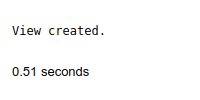
\includegraphics[scale=0.5]{./imagens/at-01.png}
						\caption{Nome dos alunos do 1 período.}
						\label{rota-1}
					\end{figure}
				\end{center}
			
						\item Dê os nomes dos professores que ministram disciplinas na Sala 2 às sextas-feiras.
						\begin{verbatim}

			SELECT DISTINCT P.PNome	AS PROFESSORES FROM PROF P, DISCIPLINA D, AULA A
			   WHERE D.DId = A.DId AND D.PId = P.PId AND A.DiaSemana = 'Sexta-Feira'
			    AND A.Sala = '1';
						\end{verbatim}
						
						\begin{center}
							\begin{figure}[H]
								\centering
								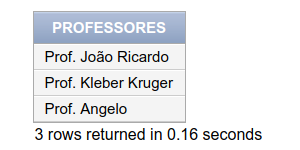
\includegraphics[scale=0.5]{./imagens/at-02.png}
								\caption{Nome dos professores.}
								\label{rota-1}
							\end{figure}
						\end{center}
					
						\item Dê os nomes dos alunos que estão matriculados em ao menos duas disciplinas distintas ministradas
						pelo mesmo professor.
					\begin{verbatim}
					SELECT DISTINCT E.ENome AS Nome_Dos_Estudantes FROM
					 ESTUDANTE E, PROF P, DISCIPLINA D1, DISCIPLINA D2, 
					 MATRICULADO M1, MATRICULADO M2 WHERE M1.DId < > M2.DId 
					 AND M1.DId = D1.DId AND M2.DId = D2.DId AND D1.PId =
					  D2.PId AND E.ENUM = M1.ENUM AND E.ENUM = M2.ENUM;
					\end{verbatim}
						\begin{center}
						\begin{figure}[H]
							\centering
								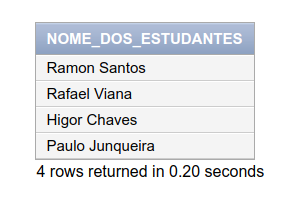
\includegraphics[scale=0.5]{./imagens/at-03.png}
							\caption{Nome dos estudantes.}
							\label{rota-1}
						\end{figure}
					\end{center}
				
								\item Encontre as idades dos alunos mais velhos do curso de Ciência da Computação ou que estejam
								matriculados em uma disciplina ministrada pelo Prof. Antônio.
							\begin{verbatim}
							SELECT MAX(E.Idade) AS MAIS_VELHO FROM ESTUDANTE E 
							WHERE (E.Curso = 'Ciência da Computação') OR E.ENUM IN 
							(SELECT M.ENUM FROM DISCIPLINA D, MATRICULADO M, PROF P 
					WHERE M.DId = D.Did AND D.PId = P.PId AND P.PNome = 'Prof. Antônio');
							\end{verbatim}
							
							\begin{center}
								\begin{figure}[H]
									\centering
									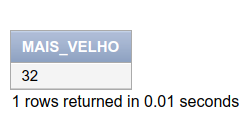
\includegraphics[scale=0.8]{./imagens/at-04.png}
									\caption{Idade dos alunos.}
									\label{rota-1}
								\end{figure}
							\end{center}
						
						
						\item Encontre os nomes das disciplinas ministradas na sala 1 ou que tenham 5 ou mais alunos
						matriculados.
						\begin{verbatim}
						SELECT (D.Dnome) AS DISCIPLINA FROM DISCIPLINA D, AULA A 
						WHERE D.DId = A.DId and A.Sala=1 AND 
						(SELECT DISTINCT COUNT (M.ENUM) FROM MATRICULADO M, ESTUDANTE E
						WHERE D.DId = M.DId AND E.ENUM=M.ENUM)>=5;
						\end{verbatim}
						
						\begin{center}
							\begin{figure}[H]
								\centering
								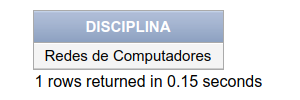
\includegraphics[scale=0.5]{./imagens/at-05.png}
								\caption{Nome das disciplinas.}
								\label{rota-1}
							\end{figure}
						\end{center}
						\item Encontre os nomes de todos os estudantes que estão matriculados em duas disciplinas que são
						ministradas no mesmo horário.
					matriculados.
					\begin{verbatim}
					SELECT DISTINCT E.ENome AS NOMES FROM ESTUDANTE E
					WHERE E.ENUM IN(SELECT M1.ENUM FROM MATRICULADO M1, MATRICULADO M2, AULA A1,
					AULA A2 WHERE M1.ENUM = M2.ENUM AND M1.Did = A1.Did AND M2.DId = A2.Did AND
					A1.Did <> A2.Did AND A1.Horario = A2.Horario);
					\end{verbatim}
					
					\begin{center}
						\begin{figure}[H]
							\centering
							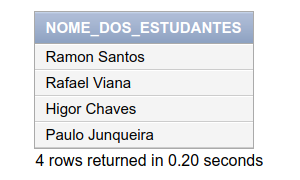
\includegraphics[scale=0.5]{./imagens/at-06.png}
							\caption{Nome dos alunos.}
							\label{rota-1}
						\end{figure}
					\end{center}
					\item Encontre os nomes de professores que ministram aulas em todas as salas onde alguma disciplina é
					ministrada.
				\begin{verbatim}
				\end{verbatim}
				
				\begin{center}
					\begin{figure}[H]
						\centering
						%	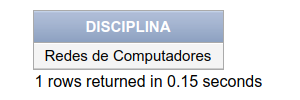
\includegraphics[scale=0.5]{./imagens/at-05.png}
						\caption{}
						\label{rota-1}
					\end{figure}
				\end{center}
				\item Encontre os nomes dos professores para os quais o total de alunos das disciplinas que eles ministram
				é inferior a 5.
			\begin{verbatim}
			
			SELECT DISTINCT P.PNome AS NOMES_PROFESSORES
			FROM PROF P
			WHERE 5 > (SELECT COUNT(M.ENUM)
			FROM MATRICULADO M, DISCIPLINA D
			WHERE M.Did = D.DId AND D.Pid = P.Pid)
			\end{verbatim}
			
			\begin{center}
				\begin{figure}[H]
					\centering
						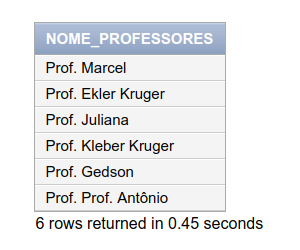
\includegraphics[scale=0.5]{./imagens/at-08.png}
					\caption{Nome dos professores.}
					\label{rota-1}
				\end{figure}
			\end{center}
			\item Imprima os períodos e as médias de idades dos alunos de cada período.
		\begin{verbatim}
		SELECT E.Periodo, AVG(E.Idade) AS Media_De_Idade FROM 
		ESTUDANTE E GROUP BY E.Periodo;
		\end{verbatim}
		
		\begin{center}
			\begin{figure}[H]
				\centering
					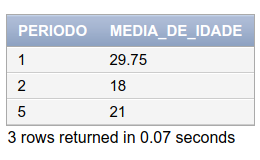
\includegraphics[scale=0.5]{./imagens/at-09.png}
				\caption{Média idade .}
				\label{rota-1}
			\end{figure}
		\end{center}
		\item O mesmo da consulta precedente, só que excluindo os alunos do 1 período.
	\begin{verbatim}SELECT E.Periodo, AVG(E.Idade) AS Media_De_Idade
	FROM ESTUDANTE E WHERE E.Periodo <> 1 GROUP BY E.Periodo;
	\end{verbatim}
	
	\begin{center}
		\begin{figure}[H]
			\centering
				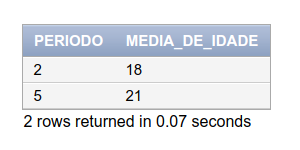
\includegraphics[scale=0.5]{./imagens/at-10.png}
			\caption{Média idade .}
			\label{rota-1}
		\end{figure}
	\end{center}
	\item Para cada professor que só ministra aulas na sala 1, imprima seu nome e o total de disciplinas que
	ele ministra.
\begin{verbatim}

\end{verbatim}

\begin{center}
	\begin{figure}[H]
		\centering
		%	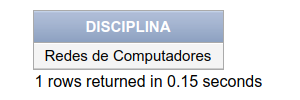
\includegraphics[scale=0.5]{./imagens/at-05.png}
		\caption{Nome dos alunos do 1\={o} período.}
		\label{rota-1}
	\end{figure}
\end{center}
	\item Encontre os nomes de alunos matriculados no maior número de disciplinas.
\begin{verbatim}
SELECT DISTINCT E.ENome AS Alunos_Com_Mais_Disciplina
FROM ESTUDANTE E WHERE E.ENUM IN
(SELECT M.ENUM FROM MATRICULADO M GROUP BY M.ENUM
HAVING COUNT(*) >= ALL (SELECT COUNT(*)
FROM MATRICULADO M1 GROUP BY M1.ENUM));
\end{verbatim}

\begin{center}
	\begin{figure}[H]
		\centering
			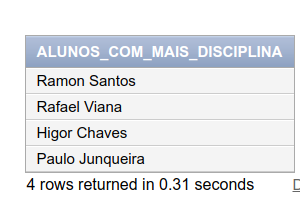
\includegraphics[scale=0.5]{./imagens/at-12.png}
		\caption{Nomes de alunos matriculados.}
		\label{rota-1}
	\end{figure}
\end{center}
	\item Encontre os nomes dos alunos que estão matriculados em todas as disciplinas.
\begin{verbatim}

\end{verbatim}

\begin{center}
	\begin{figure}[H]
		\centering
		%	\includeg\textbf{}raphics[scale=0.5]{./imagens/at-05.png}
		\caption{}
		\label{rota-1}
	\end{figure}
\end{center}
	\item Encontre os nomes dos alunos que não estão matriculados em nenhuma disciplina.
\begin{verbatim}
SELECT DISTINCT E.ENome AS Alunos FROM ESTUDANTE E
 WHERE
  E.ENUM NOT IN (SELECT M.ENUM FROM MATRICULADO M);
\end{verbatim}

\begin{center}
	\begin{figure}[H]
		\centering
			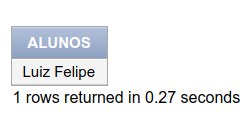
\includegraphics[scale=0.8]{./imagens/at-14.png}
		\caption{Nomes dos alunos que não estão matriculados.}
		\label{rota-1}
	\end{figure}
\end{center}
	\end{enumerate}
	
\end{document}
